\subsection{de.view.elements.map}

\rule{\textwidth}{0.4pt} 
\class{Legend}
public class Legend

\begin{minipage}{0.3\textwidth}
    \begin{figure}[H]
        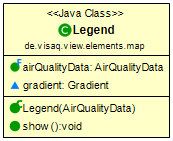
\includegraphics[scale = 0.6]{media/frontend/view/de.view.elements.map/Legend_Class.png}
    \end{figure}
    \end{minipage} \hfill
    \begin{minipage}{0.6\textwidth}
Die Legende zeigt die Farbskala für die auf der Karte angezeigten Interpolationswerte. Die Legende ändert ihre Farbwerte je nach ausgewählter Luftqualitätsdata
\end{minipage}

Attribute:
\begin{itemize} 
    \item \emph{public final AirQualityData airQualityData} Die von dem Benutzer ausgewählte Luftqualitätsdata
\end{itemize} 
Methoden:
\begin{itemize}     
    \item \emph{public Legend(AirQualityData airQualityData)} Konstruktor für die Legende mit den ausgewählten Luftqualitätsdata
    \item \emph{public void show()} Zeigt eine Legende für die Interpolationswerte auf der Karte an. Aktualisiert sich, wenn der Benutzer in der Navigationsbar eine andere Luftqualitätsdata aussucht.
\end{itemize}

\rule{\textwidth}{0.4pt} 
\class{SensorOverview}
public class SensorOverview

\begin{minipage}{0.4\textwidth}
    \begin{figure}[H]
        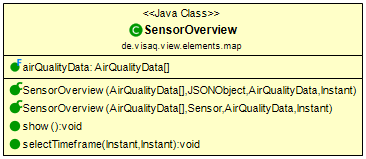
\includegraphics[scale = 0.5]{media/frontend/view/de.view.elements.map/SensorOverview_Class.png}
    \end{figure}
    \end{minipage} \hfill
    \begin{minipage}{0.4\textwidth}
SensorOverview (auch Sidebar genannt) wird benutzt um die Interpolierten Point Data auf der Karte sowie die Daten eines speziellen Sensors anzuzeigen. Es zeigt ein Diagramm mit historischen Werten an, welche von dem Benutzer individuell gewählt werden können. Außerdem werden die Gefahren von den spezifischen Arten von Luftverschmutzung angezeigt, sowie die von dem Sensor gemessenen Werte.
\end{minipage}

Attribute:
\begin{itemize} 
    \item \emph{public final AirQualityData[] airQualityData} Ein Array mit den vier AirQualityDaten
\end{itemize}
Methoden:
\begin{itemize} 
    \item \emph{public SensorOverview(AirQualityData[] airQualityData, JSONObject coordinates, AirQualityData currentAirQualityData, Instant time)} Konstruktor für die Sidebar mit den Koordinaten und der zurzeit ausgewählten Luftqualitätsdata
    \item \emph{public SensorOverview(AirQualityData[] airQualityData, Sensor sensor, AirQualityData currentAirQualityData, Instant time)}
    \item \emph{public void show()} Zeigt die Sidebar
    \item \emph{public void selectTimeframe(String start, String end)} Die von dem Benutzer ausgewählte Zeit
\end{itemize}